\documentclass[11pt]{article}
\usepackage[margin=1in]{geometry}
\usepackage{amsmath,amssymb,amsthm,booktabs,tabularx,array}
\usepackage[T1]{fontenc}
\usepackage{lmodern,microtype}
\usepackage{tikz}
\usetikzlibrary{arrows.meta}
\usepackage[colorlinks=true,linkcolor=blue,citecolor=blue,urlcolor=blue]{hyperref}
\hypersetup{pdftitle={A counterexample to Greedy Sparsest Poset consistency under restricted faithfulness},pdfauthor={Kaiwen Jin}}
\newtheorem{theorem}{Theorem}
\newtheorem{lemma}[theorem]{Lemma}
\newcommand{\po}{\operatorname{po}}
\newcommand{\clma}{\operatorname{cl}_{\mathrm{ma}}}
\newcommand{\pa}{\operatorname{pa}}
\newcommand{\spg}{\operatorname{sp}}
\newcommand{\bidir}{\leftrightarrow}
\newcommand{\indep}{\mathrel{\perp\!\!\!\perp}}
\title{A counterexample to Greedy Sparsest Poset consistency\\under restricted faithfulness}
\author{Kaiwen Jin\\\small\href{mailto:yui.ui.siki@gmail.com}{yui.ui.siki@gmail.com}}
\date{October 13, 2026}
\begin{document}
\maketitle
\begin{abstract}
The oracle consistency conjecture for Greedy Sparsest Poset asks whether
every starting graph can reach a globally sparsest graph by legitimate mark
changes and reconstruction, without increasing the edge count. We give a
counterexample under its stated Markov and restricted-faithfulness assumptions.
For a nondegenerate Gaussian distribution on six variables, an explicit
starting poset maps to an eight-edge graph whose entire reachable component
consists of three eight-edge graphs, whereas the global minimum is six.
Both applications of the poset-to-graph construction and the maximal
ancestral closure fix each of these three graphs. The Gaussian input is a
previously published example; the obstruction is established by analyzing
all possible mark changes. Exact conditional-independence and reconstruction
tables are included. The example does not address consistency under full
faithfulness.
\end{abstract}

\section{Introduction}
Ordering-based causal discovery with latent variables associates a directed
maximal ancestral graph to each partial order of the observed variables.
Bernstein, Saeed, Squires and Uhler \cite[\S\S3--4]{BS20} prove that global
minimization of the edge count identifies the true Markov-equivalence class
under restricted faithfulness. They separately conjecture that the Greedy
Sparsest Poset search can reach a global minimum from every starting point
\cite[Conjecture 1 and Algorithm 2]{BS20}. Squires and Uhler
\cite[\S4.4, p.~1803]{SU23} retain this search question.

The distinction between global minimization and reachability matters even
when all conditional independences are known exactly. We use the Gaussian
structural equation model in \cite[Figure 1, p.~4101]{BS20} and exhibit a
closed three-graph component of the prescribed search. Each graph in this
component has eight edges; a graph with six edges is an image of the same
poset construction. Thus no search depth permits an escape from the component.
The Gaussian construction is credited to \cite{BS20}; the argument below
concerns its search behavior. In particular, it does not challenge their
global sparsest-graph theorem.

\section{The search and the counterexample}\label{sec:setup}
A directed maximal ancestral graph (DMAG) has directed and bidirected edges,
at most one edge per vertex pair, no directed cycles, and no directed path
between the endpoints of a bidirected edge. On a path, an internal vertex is
a collider when both incident path edges have arrowheads at that vertex.
A path is \emph{$m$-connecting} given a set $S$ of other vertices when every
internal noncollider is outside $S$ and every internal collider has a directed
descendant in $S$, allowing itself. Absence of such a path defines
$m$-separation. Maximality requires a separating set for every nonadjacent
pair. Write $I(H)$ for the separations encoded by $H$; DMAGs are Markov
equivalent when these separation models agree.

A distribution $P$ is Markov to $G^*$ if every separation in $I(G^*)$ is a
conditional independence of $P$. Restricted faithfulness requires dependence
for every $m$-connected pair, given every $S\subseteq V\setminus\{i,j\}$,
whenever the pair is adjacent, shares a skeleton neighbor, or is the pair of
endpoints of a discriminating path. A discriminating path for $k$ has the
form $\langle i,\ldots,k,j\rangle$, at least three edges, nonadjacent
endpoints, and every vertex strictly between $i$ and $k$ is both a collider
on the path and a parent of $j$. These are the assumptions of
\cite[Definition 1]{BS20}.

For a partial order $\pi$, let
\[
D_\pi(i,j)=\{v:v\le_\pi i\ \text{or}\ v\le_\pi j\}\setminus\{i,j\}.
\]
The graph $A(\pi,P)$ joins $i,j$ if and only if
$X_i\not\indep X_j\mid X_{D_\pi(i,j)}$. It orients comparable endpoints
from the smaller to the larger and joins incomparable endpoints by a
bidirected edge. If $\po(H)$ is directed ancestry, including equality, the
map used in the conjecture is
\begin{equation}\label{eq:map}
G_\pi=\clma\bigl(A(\po(A(\pi,P)),P)\bigr).
\end{equation}
The maximal ancestral closure $\clma$ adds inseparable pairs and preserves
the separation model and ancestral orientations. We retain both applications
of $A$ and this closure in every calculation.

The search vertices are the distinct graphs $G_\pi$. A legitimate mark
change replaces one edge $a\to b$ by $a\bidir b$, or the reverse in either
orientation, while retaining DMAG status and Markov equivalence. From $H$,
the search moves to $G_{\po(H')}$ when $H'$ is obtained by such a change.
The conjecture asks for a finite path from every starting vertex to a global
edge minimum, with nonincreasing edge counts.

Let $e_1,\ldots,e_6$ be independent standard normal variables and define
\begin{equation}\label{eq:sem}
\begin{aligned}
X_1&=e_1,&X_2&=X_1+e_2,&X_3&=X_2+e_3,\\
X_4&=X_1+e_4,&X_5&=X_4+e_5,&X_6&=X_3-X_5+e_6.
\end{aligned}
\end{equation}
Denote their joint distribution by $P$. The six-edge true graph $G^*$ has
the two directed paths $1\to2\to3\to6$ and $1\to4\to5\to6$.
Let $H_1$ have directed edges $1\to2$, $2\to3$, $1\to4$, $4\to5$ and
bidirected edges $2\bidir6$, $3\bidir6$, $4\bidir6$, $5\bidir6$.
Define $H_0$ by replacing $1\to4$ in $H_1$ with $1\bidir4$, and $H_2$
by replacing $1\to2$ in $H_1$ with $1\bidir2$.

\begin{figure}[ht]
\centering
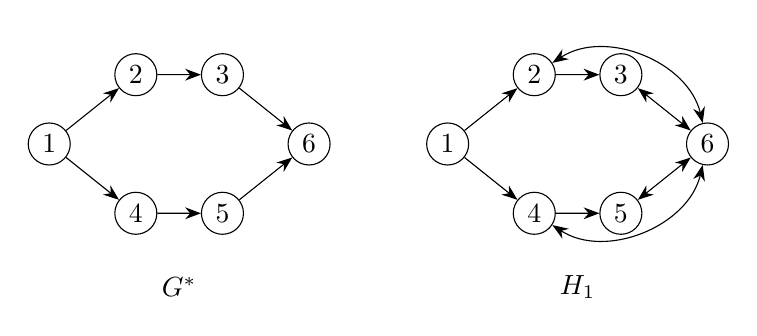
\begin{tikzpicture}[scale=1.1,vertex/.style={circle,draw,inner sep=2.5pt},
  dir/.style={-{Stealth[length=2mm]}},bi/.style={{Stealth[length=2mm]}-{Stealth[length=2mm]}}]
\foreach \shift/\prefix/\name in {0/a/G^*,4.6/b/H_1}{
  \begin{scope}[xshift=\shift cm]
  \node[vertex] (\prefix-1) at (0,0) {1};
  \node[vertex] (\prefix-2) at (1,.8) {2};
  \node[vertex] (\prefix-3) at (2,.8) {3};
  \node[vertex] (\prefix-4) at (1,-.8) {4};
  \node[vertex] (\prefix-5) at (2,-.8) {5};
  \node[vertex] (\prefix-6) at (3,0) {6};
  \draw[dir] (\prefix-1)--(\prefix-2);\draw[dir] (\prefix-2)--(\prefix-3);
  \draw[dir] (\prefix-1)--(\prefix-4);\draw[dir] (\prefix-4)--(\prefix-5);
  \node at (1.5,-1.65) {$\name$};
  \end{scope}
}
\draw[dir] (a-3)--(a-6);\draw[dir] (a-5)--(a-6);
\draw[bi] (b-3)--(b-6);\draw[bi] (b-5)--(b-6);
\draw[bi] (b-2) to[bend left=55] (b-6);
\draw[bi] (b-4) to[bend right=55] (b-6);
\end{tikzpicture}
\caption{The six-edge graph $G^*$ of the Gaussian model in
\cite[Figure 1]{BS20}, and the eight-edge graph $H_1$.
Changing one of the two edges out of vertex 1 to bidirected gives $H_0$ or $H_2$.}
\label{fig:graphs}
\end{figure}

\noindent\begin{minipage}{\textwidth}
\begin{theorem}\label{thm:main}
The distribution \eqref{eq:sem} is nondegenerate Gaussian, Markov and
restricted-faithful to the DMAG $G^*$. For the poset $\pi_0$ generated by
$1<2<3$ and $4<5$, with all unforced pairs incomparable,
$G_{\pi_0}=H_0$. Its entire reachable set in the search defined above is
$\{H_0,H_1,H_2\}$, with transitions
\begin{equation}\label{eq:component}
H_0\ \rightleftarrows\ H_1\ \rightleftarrows\ H_2.
\end{equation}
Each graph has eight edges, whereas $\min_\pi |E(G_\pi)|=6$.
Consequently the every-start oracle consistency assertion under restricted
faithfulness is false.
\end{theorem}
\end{minipage}

\section{Admissibility and reconstruction}\label{sec:admissibility}
For a positive definite Gaussian covariance $\Sigma$, set
\[
q_{ij}(S)=\Sigma_{ij}-\Sigma_{iS}\Sigma_{SS}^{-1}\Sigma_{Sj},
\qquad q_{ij}(\varnothing)=\Sigma_{ij}.
\]
Completing the square in the joint Gaussian density gives conditional
covariance $q_{ij}(S)$, so $X_i\indep X_j\mid X_S$ if and only if
$q_{ij}(S)=0$. With the elements of $S$ in increasing order, define
\begin{equation}\label{eq:minor}
N_{ij}(S)=\det\Sigma_{(i,S),(j,S)}
          =\det(\Sigma_{SS})\,q_{ij}(S).
\end{equation}
The second equality follows by eliminating the entries in the first row
against the lower rows. The empty principal determinant is 1. All other
principal determinants are positive. The same conditional-density argument
for two groups of coordinates shows that zero cross-covariance entries
give group conditional independence; hence pairwise comparisons suffice
for the Markov property of this Gaussian distribution.

From \eqref{eq:sem}, $X=Le$ with
\begin{equation}\label{eq:cov}
L=\begin{pmatrix}
1&0&0&0&0&0\\1&1&0&0&0&0\\1&1&1&0&0&0\\
1&0&0&1&0&0\\1&0&0&1&1&0\\0&1&1&-1&-1&1
\end{pmatrix},\qquad
\Sigma=LL^T=\begin{pmatrix}
1&1&1&1&1&0\\1&2&2&1&1&1\\1&2&3&1&1&2\\
1&1&1&2&2&-1\\1&1&1&2&3&-2\\0&1&2&-1&-2&5
\end{pmatrix}.
\end{equation}
The triangular matrix $L$ has diagonal 1, which proves positive definiteness.
Table~\ref{tab:minors} lists every numerator in \eqref{eq:minor} for all
15 vertex pairs and all 16 possible conditioning sets. The entries are
integer determinants of \eqref{eq:cov}.

The skeleton of $G^*$ is the cycle $1,2,3,6,5,4,1$. There are exactly two
simple paths between any pair of distinct vertices. On either path all
internal vertices other than 6 are noncolliders; vertex 6, if internal, is
a collider with no proper descendants. Thus a path is connecting precisely
when none of its other internal vertices lies in $S$ and, if 6 is internal,
$6\in S$. This rule gives Table~\ref{tab:separations}. Comparing the two
tables shows that the conditional independences of $P$ are exactly those
encoded by $G^*$ plus $X_1\indep X_6$. In particular, $P$ is Markov.
The graph is ancestral, and Table~\ref{tab:separations} provides a separator
for every nonadjacent pair, proving maximality.

The only extra independence has endpoints 1 and 6 at skeleton distance
three. They are neither adjacent nor endpoints of a length-two path.
Endpoints of a discriminating path share its first internal vertex as a
skeleton neighbor: that vertex is adjacent to the first endpoint and is a
parent of the last endpoint. Therefore 1 and 6 cannot be such endpoints.
All other connecting pairs, for every conditioning set, remain dependent by
Table~\ref{tab:minors}. This proves restricted faithfulness, with all its
conditioning-set quantifiers.

We will use the following local transformation criterion.
\begin{lemma}[Zhang--Spirtes, Lemma 1 of \cite{ZS05}]\label{lem:change}
Let $H$ be a DMAG with $a\to b$. Replacing this edge by $a\bidir b$
yields a Markov-equivalent DMAG if and only if:
\begin{enumerate}
\item there is no other directed path from $a$ to $b$;
\item every parent of $a$ is a parent of $b$, and every spouse of $a$
is a parent or spouse of $b$;
\item there is no discriminating path for $a$ ending with $a,b$.
\end{enumerate}
Here a spouse is a vertex joined by a bidirected edge.
\end{lemma}

The graph $H_1$ is ancestral, since its directed paths stay within the rooted
tree on vertices 1 through 5 and vertex 6 has no directed incident edge.
For maximality, separators for its seven nonadjacent pairs are
\[
(1,3)\mid\{2\},\quad (1,5)\mid\{4\},\quad
(1,6)\mid\varnothing,\quad
(i,j)\mid\{1\}\quad(i\in\{2,3\},\ j\in\{4,5\}).
\]
For endpoints other than 6, every path through 6 has an unconditioned
collider there; the unique path in the remaining tree is blocked by the
listed separator. A simple path from 1 to 6 first follows the directed
tree from 1 to some $v\in\{2,3,4,5\}$, then uses $v\bidir6$.
Its vertex $v$ is an unconditioned collider. This proves separation of
1 and 6 as well.

Both root-edge changes $1\to2$ to $1\bidir2$ and $1\to4$ to $1\bidir4$
in $H_1$ satisfy Lemma~\ref{lem:change}. There is no alternative directed
path; vertex 1 has neither parents nor spouses; and a discriminating path
for 1 ending at $b=2$ or 4 would require a parent of $b$ distinct from 1,
which does not exist. Thus $H_0,H_1,H_2$ are equivalent DMAGs.

Their ancestry posets $\pi_j=\po(H_j)$ are generated by
\begin{equation}\label{eq:posets}
\begin{array}{c|l}
\pi_0&1<2<3,\quad4<5\\
\pi_1&1<2<3,\quad1<4<5\\
\pi_2&2<3,\quad1<4<5.
\end{array}
\end{equation}
All unforced pairs, including those involving 6, are incomparable.
Table~\ref{tab:adjacency} gives every $D_{\pi_j}(i,j)$ and conditional
covariance for $j=0,1$, and for $\po(G^*)$. Nonzero entries produce
exactly the edges specified above, with their prescribed orientations.
Hence $A(\pi_j,P)=H_j$ for $j=0,1$, and $A(\po(G^*),P)=G^*$.
The transformation
\[
(X_1,X_2,X_3,X_4,X_5,X_6)
\longmapsto (X_1,X_4,X_5,X_2,X_3,-X_6)
\]
preserves $P$: exchange $(e_2,e_3)$ with $(e_4,e_5)$ and replace $e_6$
by $-e_6$ in \eqref{eq:sem}. It exchanges $H_0$ with $H_2$ and
preserves conditional independence, giving $A(\pi_2,P)=H_2$.
Because $\pi_j=\po(H_j)$, each second application of $A$ returns the
same graph. Maximality makes the closure the identity. Therefore
\begin{equation}\label{eq:fixed}
G_{\pi_j}=H_j\quad(j=0,1,2),\qquad G_{\po(G^*)}=G^*.
\end{equation}
Every true adjacent pair has a nonzero numerator for every conditioning set
in Table~\ref{tab:minors}. It therefore occurs in each application of $A$
for every poset, and the closure cannot remove it. Consequently every
$G_\pi$ has at least six edges, and \eqref{eq:fixed} attains this bound.

\section{The closed search component}\label{sec:component}
We now check every possible mark change. For a proposed change of
$a\bidir b$ to $a\to b$, condition 2 of Lemma~\ref{lem:change} is tested
in the hypothetical resulting directed-edge graph. If the change were
legitimate, that graph would be a DMAG and the lemma would apply in reverse.
Thus an unchanged parent or spouse violating condition 2 rules the change
out, without assuming the hypothetical graph is valid.

The following changes fail in every $H_j$; the table records an unchanged
obstruction. Nonadjacency below always refers to the common skeleton.
\begin{center}\small
\begin{tabularx}{\textwidth}{@{}lX@{}}
\toprule
Proposed change&Violation of condition 2\\\midrule
$2\to3$ to $2\bidir3$&1 is a parent of 2 in $H_0,H_1$, or a spouse
of 2 in $H_2$, but is nonadjacent to 3.\\
$4\to5$ to $4\bidir5$&1 is a spouse of 4 in $H_0$, or a parent
of 4 in $H_1,H_2$, but is nonadjacent to 5.\\
$2\bidir6$ to $2\to6$&1 is a parent or spouse of 2, but is nonadjacent to 6.\\
$3\bidir6$ to $3\to6$&$2\to3$ is present, but $2\to6$ is absent.\\
$4\bidir6$ to $4\to6$&1 is a parent or spouse of 4, but is nonadjacent to 6.\\
$5\bidir6$ to $5\to6$&$4\to5$ is present, but $4\to6$ is absent.\\
$2\bidir6$ to $6\to2$&4 is a spouse of 6, but is nonadjacent to 2.\\
$3\bidir6$ to $6\to3$&4 is a spouse of 6, but is nonadjacent to 3.\\
$4\bidir6$ to $6\to4$&2 is a spouse of 6, but is nonadjacent to 4.\\
$5\bidir6$ to $6\to5$&2 is a spouse of 6, but is nonadjacent to 5.\\
\bottomrule
\end{tabularx}
\end{center}
For the remaining two edges incident to 1, $H_1$ permits exactly the
two changes already proved legitimate. In $H_0$, changing $1\bidir4$
to $1\to4$ returns $H_1$. Changing it to $4\to1$ fails because 6 is
a spouse of 4 but is nonadjacent to 1. Changing $1\to2$ to $1\bidir2$
fails because 4 is a spouse of 1 but is nonadjacent to 2.
The exchanged argument in $H_2$ permits only $1\bidir2$ to $1\to2$,
returning $H_1$: the opposite orientation fails because 6 is a spouse of 2
nonadjacent to 1, and changing $1\to4$ to $1\bidir4$ fails because
2 is a spouse of 1 nonadjacent to 4.

There are 13 possible single mark changes in $H_0$, 12 in $H_1$, and 13
in $H_2$; these arguments cover them all, including both orientations of
each bidirected edge. The only legitimate changes are $H_0\to H_1$,
$H_1\to H_0$, $H_1\to H_2$, and $H_2\to H_1$.
Reconstruction fixes every changed graph by \eqref{eq:fixed}, proving
\eqref{eq:component}.

\begin{proof}[Completion of the proof of Theorem~\ref{thm:main}]
Section~\ref{sec:admissibility} establishes all distributional assumptions
and shows that the specified starting poset maps to $H_0$.
Every search path from $H_0$ remains among the three graphs just analyzed.
Every visited graph has eight edges, while the global minimum is six.
No path reaches a minimum, even if increasing moves were allowed, and
in particular no nonincreasing path does so.\qedhere
\end{proof}

The component also misses the true Markov-equivalence class directly:
$G^*$ separates 2 and 6 given $\{1,3\}$, whereas these vertices are adjacent
in every $H_j$. The obstruction uses the marginal cancellation
$X_1\indep X_6$, which full faithfulness would exclude. We make no
conclusion about full faithfulness, generic coefficients, alternative
search moves, or finite-sample inference.

\appendix
\section{Exact conditional-independence tables}\label{app:tables}
For each pair $i<j$, let $s_1<s_2<s_3<s_4$ be the other vertices.
Encode $S$ by $c(S)=\sum_{k:s_k\in S}2^{k-1}$, between 0 and 15.
Table~\ref{tab:minors} gives $N_{ij}(S)$, and
Table~\ref{tab:separations} gives the codes of separating sets in $G^*$.
Thus these tables can be checked directly from \eqref{eq:cov} and the
two-path rule in Section~\ref{sec:admissibility}; no enumeration of all
posets is needed. The optional accompanying Python checker uses rational
arithmetic and exhaustive simple-path separation tests to reproduce the
tables, the four fixed points, and all legitimate transitions.
\begin{table}[!ht]
\centering\small\setlength{\tabcolsep}{3pt}
\begin{tabular}{@{}lrrrrrrrrrrrrrrrr@{}}\toprule
$(i,j)$&0&1&2&3&4&5&6&7&8&9&10&11&12&13&14&15\\\midrule
$(1,2)$&1&1&1&1&2&2&1&1&5&3&3&2&4&2&2&1\\
$(1,3)$&1&0&1&0&2&0&1&0&5&1&2&0&2&0&1&0\\
$(1,4)$&1&1&2&1&1&1&2&1&5&3&4&2&3&2&2&1\\
$(1,5)$&1&1&2&1&0&0&0&0&5&2&2&1&1&0&0&0\\
$(1,6)$&0&-1&-2&-1&1&0&0&0&2&0&0&0&1&0&0&0\\
$(2,3)$&2&1&3&1&5&2&3&1&8&3&6&2&5&2&3&1\\
$(2,4)$&1&0&1&0&1&0&1&0&6&1&2&0&2&0&1&0\\
$(2,5)$&1&0&1&0&0&0&0&0&7&2&1&0&3&1&0&0\\
$(2,6)$&1&1&-1&0&3&1&0&0&5&2&0&0&3&1&0&0\\
$(3,4)$&1&0&0&0&1&0&0&0&7&2&3&1&1&0&0&0\\
$(3,5)$&1&0&0&0&0&0&0&0&9&4&5&2&5&2&3&1\\
$(3,6)$&2&2&2&1&5&2&3&1&8&4&5&2&5&2&3&1\\
$(4,5)$&2&1&3&1&5&2&3&1&8&3&6&2&5&2&3&1\\
$(4,6)$&-1&-1&-3&-1&-5&-2&-3&-1&1&0&0&0&0&0&0&0\\
$(5,6)$&-2&-2&-5&-2&-8&-4&-5&-2&-2&-1&-3&-1&-5&-2&-3&-1\\
\bottomrule\end{tabular}
\caption{All 240 almost-principal determinant numerators $N_{ij}(S)$.
The column is the conditioning-set code $c(S)$ defined above.}
\label{tab:minors}\end{table}
\begin{table}[!ht]
\centering\small
\begin{tabular}{@{}lll@{}}\toprule
$(i,j)$&Other vertices in bit order&$m$-separating codes in $G^*$\\\midrule
$(1,2)$&$3,4,5,6$&$\varnothing$\\
$(1,3)$&$2,4,5,6$&$1,3,5,7,11,13,15$\\
$(1,4)$&$2,3,5,6$&$\varnothing$\\
$(1,5)$&$2,3,4,6$&$4,5,6,7,13,14,15$\\
$(1,6)$&$2,3,4,5$&$5,6,7,9,10,11,13,14,15$\\
$(2,3)$&$1,4,5,6$&$\varnothing$\\
$(2,4)$&$1,3,5,6$&$1,3,5,7,11,13,15$\\
$(2,5)$&$1,3,4,6$&$1,3,4,5,6,7,11,14,15$\\
$(2,6)$&$1,3,4,5$&$3,6,7,10,11,14,15$\\
$(3,4)$&$1,2,5,6$&$1,2,3,5,6,7,13,14,15$\\
$(3,5)$&$1,2,4,6$&$1,2,3,4,5,6,7$\\
$(3,6)$&$1,2,4,5$&$\varnothing$\\
$(4,5)$&$1,2,3,6$&$\varnothing$\\
$(4,6)$&$1,2,3,5$&$9,10,11,12,13,14,15$\\
$(5,6)$&$1,2,3,4$&$\varnothing$\\
\bottomrule\end{tabular}
\caption{Separations in the true graph. Empty code lists mean there is
no separating set, rather than that the empty set separates. Comparing
with Table~\ref{tab:minors} leaves only the extra independence $(1,6\mid\varnothing)$.}
\label{tab:separations}\end{table}
\clearpage
\section{Reconstruction tables}
Table~\ref{tab:adjacency} lists all conditioning sets $D=D_{\po(H)}(i,j)$
and values $q=q_{ij}(D)$ needed for the first application of $A$.
Each resulting graph has the same ancestry poset and is maximal, which
also checks the second application and closure in \eqref{eq:map}.
The symmetry in Section~\ref{sec:admissibility} gives the $H_2$ table.
\begin{table}[!ht]
\centering\small\setlength{\tabcolsep}{6pt}
\begin{tabular}{@{}lrrrrrr@{}}\toprule
&\multicolumn{2}{c}{$H_0$}&\multicolumn{2}{c}{$H_1$}&\multicolumn{2}{c}{$G^*$}\\
$(i,j)$&$D$&$q$&$D$&$q$&$D$&$q$\\\midrule
$(1,2)$&$\varnothing$&$1$&$\varnothing$&$1$&$\varnothing$&$1$\\
$(1,3)$&$\{2\}$&$0$&$\{2\}$&$0$&$\{2\}$&$0$\\
$(1,4)$&$\varnothing$&$1$&$\varnothing$&$1$&$\varnothing$&$1$\\
$(1,5)$&$\{4\}$&$0$&$\{4\}$&$0$&$\{4\}$&$0$\\
$(1,6)$&$\varnothing$&$0$&$\varnothing$&$0$&$\{2,3,4,5\}$&$0$\\
$(2,3)$&$\{1\}$&$1$&$\{1\}$&$1$&$\{1\}$&$1$\\
$(2,4)$&$\{1\}$&$0$&$\{1\}$&$0$&$\{1\}$&$0$\\
$(2,5)$&$\{1,4\}$&$0$&$\{1,4\}$&$0$&$\{1,4\}$&$0$\\
$(2,6)$&$\{1\}$&$1$&$\{1\}$&$1$&$\{1,3,4,5\}$&$0$\\
$(3,4)$&$\{1,2\}$&$0$&$\{1,2\}$&$0$&$\{1,2\}$&$0$\\
$(3,5)$&$\{1,2,4\}$&$0$&$\{1,2,4\}$&$0$&$\{1,2,4\}$&$0$\\
$(3,6)$&$\{1,2\}$&$1$&$\{1,2\}$&$1$&$\{1,2,4,5\}$&$1$\\
$(4,5)$&$\varnothing$&$2$&$\{1\}$&$1$&$\{1\}$&$1$\\
$(4,6)$&$\varnothing$&$-1$&$\{1\}$&$-1$&$\{1,2,3,5\}$&$0$\\
$(5,6)$&$\{4\}$&$-1$&$\{1,4\}$&$-1$&$\{1,2,3,4\}$&$-1$\\
\bottomrule\end{tabular}
\caption{Exact adjacency calculations for $H_0$, $H_1$, and $G^*$.
An edge occurs precisely when $q\ne0$, with orientation determined by the poset.}
\label{tab:adjacency}\end{table}

\begin{thebibliography}{9}
\bibitem{BS20}
D.~I. Bernstein, B.~Saeed, C.~Squires and C.~Uhler.
\newblock Ordering-Based Causal Structure Learning in the Presence of Latent Variables.
\newblock In \emph{Proceedings of the Twenty Third International Conference
on Artificial Intelligence and Statistics}, Proceedings of Machine Learning
Research \textbf{108}, 4098--4108, 2020.
\newblock \url{https://proceedings.mlr.press/v108/bernstein20a.html}.

\bibitem{SU23}
C.~Squires and C.~Uhler.
\newblock Causal Structure Learning: A Combinatorial Perspective.
\newblock \emph{Foundations of Computational Mathematics} \textbf{23},
1781--1815, 2023.
\newblock \url{https://doi.org/10.1007/s10208-022-09581-9}.

\bibitem{ZS05}
J.~Zhang and P.~Spirtes.
\newblock A transformational characterization of Markov equivalence for
directed acyclic graphs with latent variables.
\newblock In \emph{Proceedings of the Twenty-First Conference on Uncertainty
in Artificial Intelligence}, 2005, \S2.2, Lemma~1.
\newblock \url{https://arxiv.org/abs/1207.1419v1}.
\end{thebibliography}

\paragraph{AI use.}
OpenAI Codex assisted with the search for the obstruction, exact-arithmetic
code, proof development, source checking, and manuscript preparation.
AI assistance does not constitute human or formal verification.
Independent mathematical review is requested.
\end{document}
